\documentclass{article}

\usepackage[hidelinks]{hyperref}

\usepackage{graphicx}
\usepackage[export]{adjustbox}
% sudo dnf install texlive-adjustbox
\graphicspath{{images/}}
% for graphics
\usepackage{float}

\usepackage{amsmath}
% for more advanced math equations

\usepackage{parskip}
% enter a vertical space between paragraphs and skip the indentation

\usepackage{tikz}
\usepackage{tikz-qtree}
% sudo dnf install texlive-tikz-qtree

\usepackage{geometry}

\usepackage{listings}
\lstset{
    frame=single,
    breaklines=true,
    postbreak=\raisebox{0ex}[0ex][0ex]{\ensuremath{\color{blue}\hookrightarrow\space}}
}

\usepackage{polyglossia}
\setdefaultlanguage[variant=modern]{greek}
\setotherlanguage{english}
\newfontfamily\greekfont{Open Sans Light}
\newfontfamily\greekfonttt{Inconsolata}
\newfontfamily\englishfont{Open Sans Light}
\newfontfamily\englishfonttt{Inconsolata}

\usepackage{datetime2}
% sudo dnf install texlive-datetime2-english
% sudo dnf install texlive-datetime2-greek
\DTMnewdatestyle{monthyear}{%
    \renewcommand*{\DTMdisplaydate}[4]{\DTMgreekmonthname{##2}, ##1}%
    \renewcommand*{\DTMDisplaydate}{\DTMdisplaydate}%
}
\DTMsetdatestyle{monthyear}
\renewcommand*{\DTMgreekmonthname}[1]{%
    \ifcase#1
    \or
    Ιανουάριος%
    \or
    Φεβρουάριος%
    \or
    Μάρτιος%
    \or
    Απρίλιος%
    \or
    Μάιος%
    \or
    Ιούνιος%
    \or
    Ιούλιος%
    \or
    Αύγουστος%
    \or
    Σεπτέμβριος%
    \or
    Οκτόβριος%
    \or
    Νοέμβριος%
    \or
    Δεκέμβριος%
    \fi
}

\usepackage{siunitx}

\DeclareMathOperator*{\argmax}{argmax}
% declase the math operator argmax which can also have a subscript

\title{Επίλυση του Knapsack Problem\\με Χρήση Γενετικού Αλγορίθμου}
\date{\DTMtoday}
\author{Γκαντίδης Χρήστος 56483 \\ email: \href{mailto:chrigkan@ee.duth.gr}{chrigkan@ee.duth.gr}}

\begin{document}
\pagenumbering{gobble}
% don't number first page
\maketitle
\newpage

\tableofcontents
\newpage

\pagenumbering{arabic}

\section{Εισαγωγή}

Το Knapsack Problem είναι ένα πρόβλημα εύρεσης του βέλτιστου συνδυασμού: Έχοντας
ένα σύνολο πακέτων, το καθένα από τα οποία έχει μια αξία και ένα μέγεθος, βρες
τον συνδυασμό των πακέτων που πρέπει να επιλεγούν, ώστε να μεγιστοποιείται η
συνολική τους αξία, υπό την προϋπόθεση ότι το συνολικό μέγεθος των πακέτων δεν
ξεπερνάει το μέγεθος του σακιδίου μέσα στο οποίο θα τοποθετηθούν τα πακέτα.

Το πρόβλημα αυτό αναφέρεται επίσης και ως 0-1 Knapsack Problem καθώς το κάθε
πακέτο είτε θα βρίσκεται μέσα στο σακίδιο είτε όχι. Επίσης το κάθε πακέτο δεν
μπορεί να σπάσει σε μικρότερα κομμάτια και δεν μπορεί να τοποθετηθεί πάνω από
μία φορά στο σακίδιο.

Σε μαθηματική μορφή το πρόβλημα μπορεί να εκφραστεί και ως:
\begin{align*}
    &\argmax_{S}\left(\sum_{p \in S}\textit{value}(p)\right)\\
    \text{έτσι ώστε } &\sum_{p \in S}\textit{size}(p) \leq \textit{knapsackLimit}
\end{align*}

\section{Εξαντλητικός Αλγόριθμος (Bruteforce)}

Μια πρώτη σκέψη για την επίλυση του προβλήματος, θα ήταν να πάρουμε όλους τους
πιθανούς συνδυασμούς με τους οποίους μπορούμε να επιλέξουμε ένα σύνολο $S$ από
πακέτα, από $\textit{numPackets}$ συνολικά πακέτα.

Μιας και κάθε πακέτο $p$ είτε θα ανήκει είτε όχι στο σύνολο $S$ (0-1), είναι
φανερό πως υπάρχουν $2^{\textit{numPackets}}$ τέτοιοι συνδυασμοί. Από αυτούς
τους συνδυασμούς κρατάμε μόνο αυτούς οι οποίοι δεν ξεπερνούν σε συνολικό μέγεθος
το μέγεθος του σακιδίου \textit{knapsackLimit}, και έπειτα βρίσκουμε τον
συνδυασμό με την μέγιστη συνολική αξία.

Βλέπουμε λοιπόν πως η πολυπλοκότητα αυτού του αλγορίθμου και σε υπολογισμούς και
σε μνήμη είναι $\mathcal{O}\left(2^{\textit{numPackets}}\right)$, αυξάνεται
δηλαδή εκθετικά με το πλήθος των πακέτων.

\section{Δυναμικός Προγραμματισμός (Dynamic Programing)}

Η επόμενη σκέψη είναι μήπως μπορούμε να βρούμε την βέλτιστη λύση με μικρότερη
πολυπλοκότητα από την εκθετική, και εδώ έρχεται για βοήθεια ο Δυναμικός
Προγραμματισμός.

Ας θεωρήσουμε πως το σύνολο $S$ αποτελεί την βέλτιστη λύση από ένα πλήθος $n$
πακέτων. Τότε, κάθε ένα από τα $n$ πακέτα μπορεί να βρίσκεται σε δύο
καταστάσεις: είτε θα ανήκει στο $S$ είτε όχι. Έτσι η μέγιστη αξία των $n$
πακέτων σε ένα σακίδιο μεγέθους $W$, είναι το μέγιστο από τις ακόλουθες δύο
αξίες:

\begin{enumerate}
    \item Η μέγιστη αξία που μπορεί να βρεθεί για $n-1$ πακέτα σε ένα σακίδιο
            μεγέθους $W$ (δηλαδή το $n$ πακέτο δεν ανήκει στο $S$)
    \item Η μέγιστη αξία που μπορεί να βρεθεί για $n-1$ πακέτα σε ένα σακίδιο
            μεγέθους $W-\textit{size}(n)$ (δηλαδή το $n$ πακέτο ανήκει στο $S$)
\end{enumerate}

Βλέπουμε λοιπόν πως προκύπτει μια αναδρομική σχέση από την οποία μπορούμε να
βρούμε την μέγιστη αξία για ένα πλήθος $n$ πακέτων και ένα σακίδιο μεγέθους $W$.

Έστω ότι έχουμε αριθμό πακέτων $\textit{numPackets}=3$ με βάρη πακέτων
$\textit{weights}[]=\{1, 1, 1\}$ και μέγεθος σακιδίου
$\textit{knapsackLimit}=2$. Έστω επίσης $K(n, W)$ η παραπάνω αναδρομική
συνάρτηση, η οποία δέχεται ως είσοδο τον αριθμό του πακέτου προς εκτίμηση $n$,
και το εναπομείναν μέγεθος μέσα στο σακίδιο $W$.

Κατά την εκτέλεση της συνάρτησης $K$ προκύπτει το ακόλουθο δυαδικό δέντρο, όπου
κάθε αριστερός κλάδος σημαίνει πως το $n$ πακέτο δεν ανήκει στο $S$, ενώ
κάθε δεξιός κλάδος σημαίνει πως το $n$ πακέτο ανήκει στο $S$.

\begin{center}
    \begin{tikzpicture}
    \Tree   [.K(3,2) [.K(2,2) [.K(1,2) [.K(0,2) ] [.K(0,1) ] ] [.K(1,1) [.K(0,1) ] [.K(0,0) ] ] ] [.K(2,1) [.K(1,1) [.K(0,1) ] [.K(0,0) ] ] K(1,0) ] ]
    \end{tikzpicture}
\end{center}

Διαπιστώνουμε πως κάποια υπο-δέντρα επαναλαμβάνονται, άρα αν χρησιμοποιήσουμε
Δυναμικό Προγραμματισμό ώστε να αποθηκεύουμε την τιμή που επιστρέφει η συνάρτηση
για την συγκεκριμένη είσοδο, δεν χρειάζεται να την υπολογίσουμε ξανά.

Αν αντί για την συνάρτηση $K$ χρησιμοποιήσουμε έναν πίνακα με διαστάσεις
\begin{equation*}
\left[\textit{numPackets}+1 \times \textit{knapsackLimit}+1\right]
\end{equation*}
όπου στην γραμμή $i$ και στην στήλη $j$ αποθηκεύουμε την βέλτιστη τιμή που
μπορεί να βρεθεί, εξαρτώμενη από το $i$ πακέτο με $j$ εναπομείναντα χώρο στο
σακίδιο, μπορούμε να λύσουμε το πρόβλημα με πολυπλοκότητα και σε υπολογισμούς
και σε μνήμη $\mathcal{O}\left(\textit{numPackets} \cdot
\textit{knapsackLimit}\right)$.

Αν και πλέον το πρόβλημα λύνεται σε πολυωνυμικό χρόνο, η πολυπλοκότητα εξαρτάται
πλέον από το μέγεθος του σακιδίου, το οποίο μπορεί να αποτελέσει πρόβλημα στην
περίπτωση που έχουμε να λύσουμε ένα πολύ εύκολο πρόβλημα.

Για παράδειγμα με αριθμό πακέτων $\textit{numPackets} = 1$ και μέγεθος σακιδίου
$\textit{knapsackLimit} = 1000$, η bruteforce προσέγγιση θα υπολόγιζε την
βέλτιστη λύση σε 2 βήματα ενώ ο αλγόριθμος με Δυναμικό Προγραμματισμό σε $1000$
βήματα.

\section{Γενετικός Αλγόριθμος (Genetic Algorithm)}

Την λύση έρχεται να μας δώσει η χρήση Γενετικών Αλγορίθμων.

Ο Γενετικός Αλγόριθμος που χρησιμοποιούμε χρησιμοποιεί οντότητες που η κάθε μία
αναπαρίσταται ως ένα δυαδικό διάνυσμα μήκους \textit{numPackets}. Είναι δυαδικό
καθώς σε κάθε θέση $i$ του διανύσματος έχουμε 1 ή 0 που αντιπροσωπεύει την
συμμετοχή ή όχι αντίστοιχα του $i$ πακέτου σε αυτήν την οντότητα.

Κάθε οντότητα αποτελεί μια πιθανή λύση του προβλήματος και σκοπός του γενετικού
αλγορίθμου είναι να εντοπίσει την οντότητα που παράγει την μέγιστη δυνατή
συνολική αξία.

Για να τρέξουμε το πρόγραμμα εκτελούμε το script \textit{gaKnapsack} το οποίο με
την σειρά του θα μας ρωτήσει ποιο πρόβλημα θέλουμε να λύσει. Το πρόβλημα που
ανατέθηκε στο μάθημα είναι το $01$ αλλά υπάρχουν άλλα $8$, με το πρόβλημα $09$
να αποτελεί παράδειγμα στο οποίο ο γενετικός αλγόριθμος ξεχωρίζει σε σχέση με
τον Δυναμικό Προγραμματισμό στην ταχύτητα εκτέλεσης.

Σε περιπτώσεις που το πρόβλημα είναι αρκετά εύκολο ο Γενετικός Αλγόριθμος
πιθανώς να χρειαστεί περισσότερο χρόνο από ότι ο αλγόριθμος Δυναμικού
Προγραμματισμού εξαιτίας των αρχικοποιήσεων που πρέπει να γίνουν για να επιλυθεί
το πρόβλημα.

Μια πιθανή έξοδος για την επίλυση του προβλήματος $01$ είναι η ακόλουθη:

\lstinputlisting{outputs/out_prob_01.txt}

με τον Γενετικό Αλγόριθμο να υπολογίζει τα ακόλουθα ελάχιστα σκορ σε κάθε γενιά:

\begin{figure}[H]
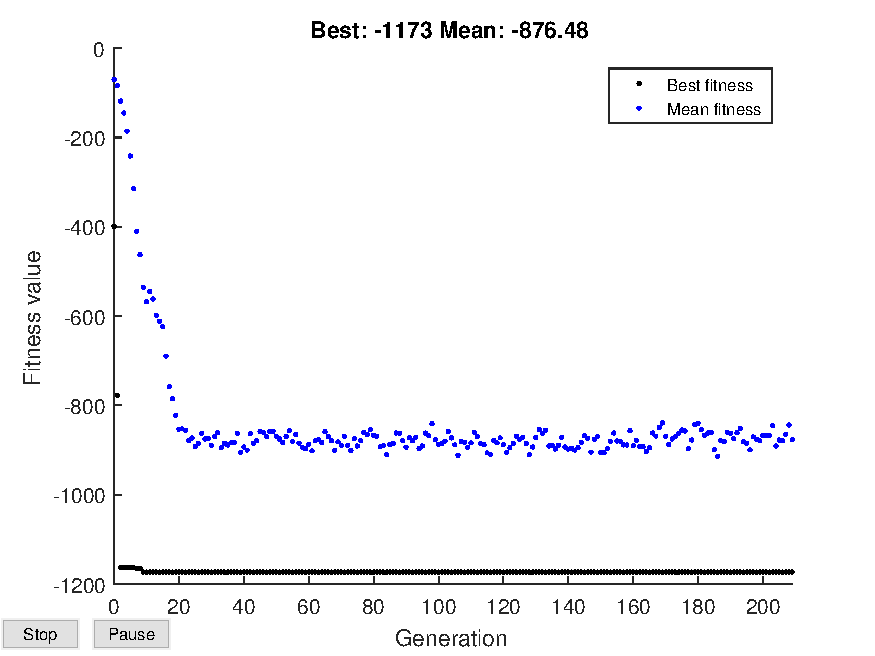
\includegraphics[max height = 0.5\textheight]{Fitness_vs_Generation_prob_01}
\centering
\caption{Fitness vs Generation prob-01}
\centering
\end{figure}

Μια πιθανή έξοδος για την επίλυση του προβλήματος $09$ είναι η ακόλουθη:

\lstinputlisting{outputs/out_prob_09.txt}

με τον Γενετικό Αλγόριθμο να υπολογίζει τα ακόλουθα ελάχιστα σκορ σε κάθε γενιά:

\begin{figure}[H]
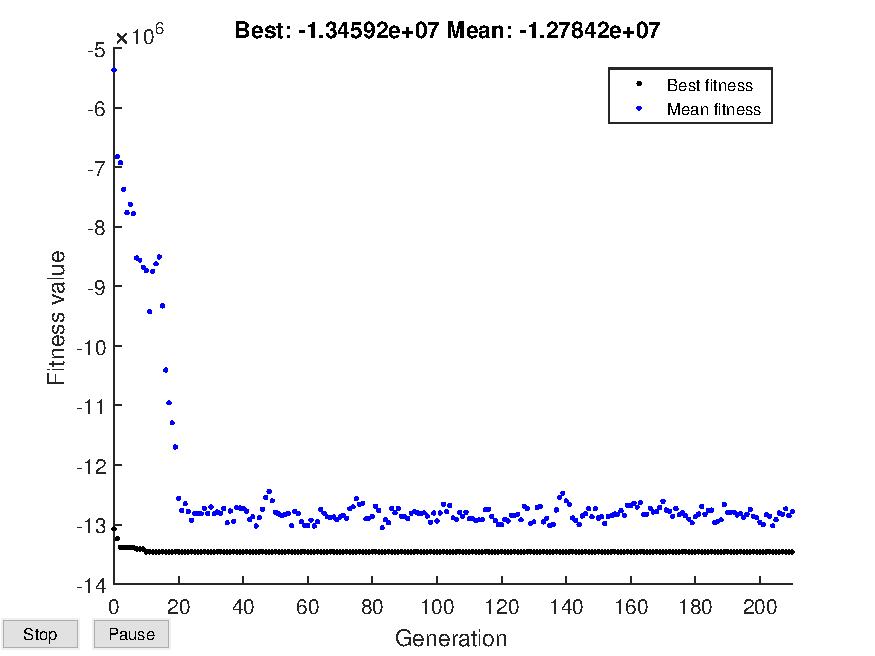
\includegraphics[max height = 0.5\textheight]{Fitness_vs_Generation_prob_09}
\centering
\caption{Fitness vs Generation prob-09}
\centering
\end{figure}
\subsection{Συνάρτηση Αρχικού Πληθυσμού (Creation Function)}

Για την δημιουργία του αρχικού πληθυσμού του προβλήματος χρησιμοποιείται η
συνάρτηση \textit{knapsackCreationFcn}.

Οι πρώτες $\textit{numPackets}$ οντότητες αρχικοποιούνται ως ένας ταυτοτικός
πίνακας διαστάσεων
\begin{equation*}
\left[\textit{numPackets} \times \textit{numPackets}\right]
\end{equation*}
κάνοντας έτσι την $i$ οντότητα να περιλαμβάνει μόνο το $i$ πακέτο. Έτσι είμαστε
σίγουροι πως ακόμη κι αν χωράει μόνο ένα πακέτο μέσα στο σακίδιο έχουμε μια
οντότητα η οποία θα ικανοποιεί αυτήν την συνθήκη.

Οι υπόλοιπες οντότητες παράγονται τυχαία ακολουθώντας ομοιόμορφη κατανομή, έτσι
ώστε σε περίπτωση που το σακίδιο χωράει πολλά πακέτα, να έχουμε οντότητες οι
οποίες κατά μέσο όρο περιλαμβάνουν τα μισά πακέτα. Έτσι έχουμε καλύψει και τις
δύο περιπτώσεις: και μικρό και μεγάλο σακίδιο.

\subsection{Συνάρτηση Μετάλαξης (Mutation Function)}

Για την μετάλλαξη του πληθυσμού χρησιμοποιείται η συνάρτηση του MATLAB
\textit{mutationuniform}, η οποία για κάθε οντότητα του πληθυσμού, επιλέγει ένα
ποσοστό των γονιδίων της οντότητας, και με πιθανότητα 0.01 αλλάζει την τιμή σε 0
ή 1, χωρίς να λαμβάνει υπόψη την τωρινή τιμή του γονιδίου.

\subsection{Συνάρτηση Διασταύρωσης (Crossover Function)}

Για την διασταύρωση των οντοτήτων του πληθυσμού χρησιμοποιείται η συνάρτηση του
MATLAB \textit{crossoverscattered}, η οποία παράγει μια τυχαία δυαδική μάσκα,
και παράγει 2 απογόνους για κάθε 2 γονείς.

Ο πρώτος απόγονος έχει τα γονίδια του πρώτου γονέα στις θέσεις που η μάσκα έχει
την τιμή 1 και τα γονίδια του δεύτερου γονέα στις θέσεις που η μάσκα έχει την
τιμή 0. Ο δεύτερος απόγονος παράγεται χρησιμοποιώντας την αντίθετη μάσκα.

\subsection{Συνάρτηση Καταλληλότητας (Fitness Function)}

Για την κατάταξη των οντοτήτων χρησιμοποιείται η συνάρτηση
\textit{knapsackFitnessFcn}, η οποία επιστρέφει ως σκορ της κάθε οντότητας, το
αντίθετο του αθροίσματος των αξιών των πακέτων που είναι ενεργά σε αυτήν την
οντότητα. Ο λόγος που χρησιμοποιείται το αντίθετο του αθροίσματος των αξιών και
όχι το ίδιο το άθροισμα, είναι γιατί ο γενετικός αλγόριθμος προσπαθεί να
ελαχιστοποιήσει την συνάρτηση καταλληλότητας, οπότε κάνοντας το άθροισμα
αρνητικό θα βρούμε την λύση με την πιο αρνητική συνολική αξία, η οποία όμως θα
είναι η μέγιστη κατά απόλυτη τιμή.

Σε περίπτωση που το άθροισμα των μεγεθών των πακέτων που είναι ενεργά σε αυτήν
την οντότητα ξεπερνά το μέγεθος του σακιδίου (\textit{knapsackLimit}), η
οντότητα έχει μηδενικό σκορ.

\subsection{Συνθήκες Τερματισμού (Stopping Criteria)}

Ο Γενετικός Αλγοριθμός προσπαθεί να μειώσει την Συνάτρηση Καταλληλότητας μέχρι
το ελάχιστο σκορ όλου του πληθυσμού να παραμείνει σταθερό για 200 γενιές. Έτσι
πετυχαίνουμε μια αρκετά καλή λύση (συνύθως την βέλτιστη) σε αρκετά μικρό χρόνο
($<$\SI{20}{\second}).

\section{Συμπεράσματα}

Αν και ο Γενετικός Αλγόριθμος δεν συγκλίνει ντετερμινιστικά στην βέλτιστη λύση,
είναι κατάληλος για περιπτώσεις που το μέγεθος του σακιδίου είναι πολύ μεγάλο, ή
για περιπτώσεις που μια καλή προσέγγιση της βέλτιστης λύσης είναι αρκετή.

Όπως βλέπουμε για παράδειγμα στην έξοδο του προβλήματος $09$, αν και ο Γνετικός
Αλγόριθμος δεν έχει βρει την βέλτιστη λύση (\num{13459221} vs \num{13549094}),
έχει βρει μια λύση πολύ κοντά στην βέλτιστη, και σε χρόνο πάνω από 20 φορές
μικρότερο από ότι ο Δυναμικός Προγραμματισμός (\SI{12.022}{\second} vs
\SI{271.940}{\second}).

\end{document}
